\chapter{Convolutional Neural Network}

  The alternative to handcrafted features that is gaining huge attention in the recent years is the possibility to let the machine learn the best features to represent the image. In the domain of image processing the learning of the features is mainly done through a model called Convolutional Neural Network (CNN). Convolutional neural networks are models inspired by how the brain works and how neurons interact between each other. They are made of successive layers of neurons, each of them aggregating the results from the preceding layer in order to compute more abstract features. The succession of layer is the reason why such algorithms are know as deep learning methods. Convolutional neural network was inspired by the neocognitron proposed by Kunihiko Fukushima in the 1980s \cite{fukushima1980neocognitron}. It was the first attempt to mimic the animals visual cortex. Early paper \cite{hubel1959receptive} had shown that the cortex of animals was made of different neurons. The neurons located downstream in the visual recognition process are responsible for the extraction of specific patterns within their receptive fields and neurons located upstream in the process aggregate these results and are invariant to specific location of the patterns. Accordingly the neocognitron consist of multiple types of cells, the most important of which are called S-cells and C-cells. The purpose of S-cells is to extract local features which are integrated gradually and classified in the higher layers. However the neocognitron lacked a proper supervised training algorithm. This algorithm was found by Yann LeCun and is known as backpropagation, abbreviation for backward propagation of errors. Backpropagation used in conjunction with an optimization method such as gradient descent has been successfully applied in 1989 to recognize handwritten digit recognition \cite{lecun1989backpropagation}. With the rise of efficient GPU computing a second breakthrough was achieved in 2012 by Geoffrey Hinton and his team which designed a convolutional neural network known as AlexNet \cite{krizhevsky2012imagenet} that achieved state-of-the-art performance on the Imagenet dataset.

  As opposed to handcrafted features convolutional neural networks has the advantages to require very little if not preliminary knowledge of the domain at hand. For instance, when using a Visual Bag-Of-Words representation for images, one has to choose between different detectors which one will be the more efficient for the task. This choice depend obviously of the underlying problem. As for convolutional  neural networks the domain knowledge is used to finely tune the parameters of the model but it is also often achieved through trial and errors. Prior knowledge can also be put into the network by designing appropriate connectivity, weights constraints and neuron activation function. In any case it is less intrusive than handcrafted features. Another benefits of convolutional neural network is their ability to learn more discriminative features. Both in the review of Chatfield and all \cite{chatfield2014return} and in the study of Zhang and all \cite{zhang2007local} they show better performance than traditional shallow methods. Drawbacks of convolutional neural networks include their complexity, the substantial amount of data and the computational resources required to train it effectively.

  \section{Design}

  The complexity of convolutional neural network reside mostly in their design and in the different layers that the network is made of. The figure \ref{convnet} illustrate a very simple convolutional neural network. It is made of the succession of two convolutional layers with pooling layers and is followed by a fully connected layer. As for the neocognitron the first layers that is the convolutional layers and the pooling layers are responsible for the extraction of local features. Specifically the convolutional layers learn to recognize different patterns and the pooling layers gradually ensure that the network is invariant to the location of these patterns. Fully connected layers enable to map this low level features to more abstract concepts. Below is a detailed description of the different layers one can find in a network.

  \begin{figure}[h]
    \centering
      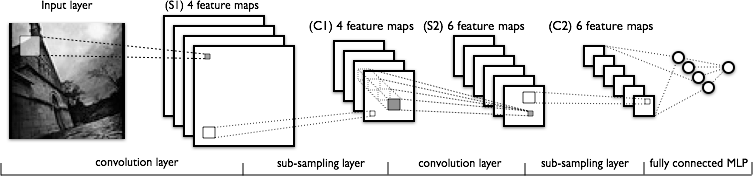
\includegraphics[width=1\textwidth]{images/convnet.png}
      \caption{A Convolutional Neural Network}
      \label{convnet}
  \end{figure}

    \subsection{Convolutional Layers} \\

    Convolutional layers are the core of convolutional neural networks. The figure \ref{convlayer} represent a convolutional layer made of four learnable linear filters or kernels. Each perform a convolution on the preceding layer. That is each filter is slid across the width and the height of the preceding layer. The output of the convolution of one filter is called a feature map. Formally we have : \[ h^k_i_j = (W^k * x)_i_j + b^k \] where \( h^k\) denote the k-th feature map, \( W^k \) and \( b^k \) the associated filter and bias and \( x \) the inputs.

    \begin{wrapfigure}{r}{0.5\textwidth}
      \begin{center}
        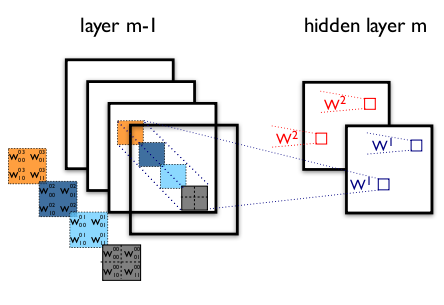
\includegraphics[width=0.48\textwidth]{images/conv_layer.png}
      \end{center}
      \caption{A Convolutional Layer}
      % \vspace{-80pt}
      \label{convlayer}
    \end{wrapfigure}

    It results of this operations that all neurons in a feature map share the same weights but have different receptive fields that is they look at different regions from the preceding layer. Thus neurons in a same feature map act as replicated features detectors able to detect a pattern at any location. Adjacent neurons in different features map share the same receptive field but the different filters learning different weights each feature map learn to detect different patterns. The exact nature of the patterns detected is hard to know and might not be easily interpretable for humans. \\
    Following the convolution each neuron is the input to an activation function that determine the final output of the layer. Different activation functions can be used such as the binary function, the logistic function, the hyperbolic tangent function but most commonly used activation function is the rectifier function. This function is defined as \( f(x) = max(0,x) \) and has been argued to be the more biologically plausible \cite{glorot2011deep}.
    \\
    Using convolutional layers before fully connected layers present many advantages. First it enable to take the spatial structure of the image into account. In fully connected layers neurons are joined to all the neurons of the previous layers thus they treat pixels which are far apart and close together exactly the same way whereas neurons in convolutional layers are only joined to neighboring neurons from the preceding layers. Also it enable to greatly reduce the number of parameters to learn by the network. For example if an image is of size 200*200*3 a single fully connected layer would have to learn \( 200*200*3 = 120,000 \) weights whereas a single convolutional layer with 50 different filters of size 5*5*3 only has to learn \( 50*5*5*3 = 3750 \) weights.

    \subsection{Pooling Layers}

    Pooling layers are common between two convolutional layers. They perform a form of non-linear down-sampling. They partition the previous layer into, overlapping or not, rectangular regions and for each region compute a unique output. It enable to get a small amount of translational invariance each time they are used.

    \begin{wrapfigure}{l}{0.5\textwidth}
      \begin{center}
        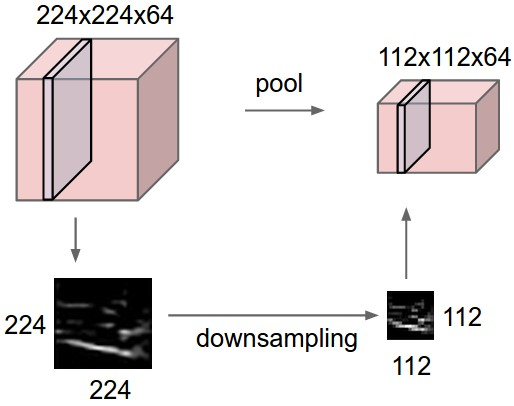
\includegraphics[width=0.48\textwidth]{images/pool_layer.jpeg}
      \end{center}
      \caption{A Pooling Layer}
      % \vspace{-40pt}
    \end{wrapfigure}

    Most of the time the function used by pooling layer is max-pooling that compute the maximum of the underlying region but average-pooling (compute the average of the underlying regions) or L2-norm pooling can also be used. By pooling the exact locations of the features are lost but relative locations, which are the most important, are preserved. Pooling layers are useful to progressively reduce the spatial size of the feature maps, thus the number of parameters and prevent overfitting. \\

    \subsection{Local Response Normalization Layer}

    Local Response Normalization Layer can be found especially in the AlexNet network \cite{krizhevsky2012imagenet}. it performs a normalization between neurons from adjacent kernels. The idea is to suppress the activity of a hidden neuron if nearby neurons in adjacent feature maps have stronger activities. Indeed if a pattern is detected with low intensity it becomes not so relevant if strong patterns are detected around. The authors argue that it helps to increase the performance of the network however another study \cite{simonyan2014very} report that performance improvement was rarely achieved by adding local response normalization layer and that it even lead to to increased memory consumption and computation time. More generally this kind of layer is not reused in subsequent works.

    \subsection{Fully Connected Layers} \\

    The following layers of a convolutional neural network are the ones that we can find in a traditional multi-layer perceptrons that is one or more successions of fully connected layers. Fully Connected Layers are called this way because the neurons of these layers are connected to all the neurons of the layer below. In a convolutional neural network the feature maps of the last convolutional layer is vectorized and fed into fully connected layers. As for convolutional layer an activation function is used. If we suppose that rectifier units are used then we formally have : \[ y_j = max(0, z_j) \quad with \quad z_j = b + \sum_{i} W_i_j * x_i \] where \( y_j \) is the output of the j-th neurons of the layer, \( W \) is the weights matrix for this layer and b is the associated bias.
    \\

    \subsection{Loss Layer}

    The loss layer specifies how the network penalize the deviation between the predicted and true labels and is obviously the last layer in the network. The layer usually implements the softmax function that take a features vector as input and force the outputs to sum to one so they can represent a probability distribution across discrete mutually exclusive classes : \[ y_i = \dfrac{e^{z_i}}{\sum_{j} e^{z_j}} \]
    The cost function associated with the softmax function is the cross-entropy function : \[ E = -\sum_{j} t_j*log(y_j) \] where \( t_j \) is the target value and \( y_j \) is the predicted value.

  \section{Training}

  The training of a network is done through the backprogation algorithm which will be explained shortly. One problem, due to the fact that convolutional neural network are able to learn complex mathematic model, is that they can easily overfit. To prevent this from happening one can either limit the number of hidden layer and the number of units per layer or stop the learning early but several more advanced methods have been proposed that we will discuss thereafter.

  \subsection{Backpropagation and Gradient Descent}

  Gradient descent is an optimization algorithm to find the local minimum of a function. In the case of machine learning it enable to find the minimum of the cost function by applying the delta rule : \[ W_i_j = W_i_j - \alpha * \nabla E(W_i_j) \]
  where \( W_i_j \) is the weight between the node i and j, \( \alpha \) is the learning rate and \( \nabla E(W_i_j) \) is the gradient of the cost function with respect to the weight \( W_i_j \).

  \begin{figure}[H]
  \centering
  \definecolor{ffqqqq}{rgb}{1.,0.,0.}
  \begin{tikzpicture}[line cap=round,line join=round,>=triangle 45,x=1.0cm,y=1.0cm, scale=0.5]
    \draw[->,color=black] (-5.563020881178121,0.) -- (9.725772242000257,0.);
    \foreach \x in {-5.,-4.,-3.,-2.,-1.,1.,2.,3.,4.,5.,6.,7.,8.,9.}
    \draw[shift={(\x,0)},color=black] (0pt,2pt) -- (0pt,-2pt);
    \draw[color=black] (9.494998006178697,0.05769355895539008) node [anchor=south west] { W};
    \draw[->,color=black] (0.,-4.425829974358826) -- (0.,4.891679796936672);
    \foreach \y in {-4.,-3.,-2.,-1.,1.,2.,3.,4.}
    \draw[shift={(0,\y)},color=black] (2pt,0pt) -- (-2pt,0pt);
    \draw[color=black] (0.07211694869423764,4.574365222682027) node [anchor=west] { E};
    \clip(-5.563020881178121,-4.425829974358826) rectangle (9.725772242000257,4.891679796936672);
    \draw [rotate around={27.99302990476193:(1.6367377401020933,0.37867809598019914)}] (1.6367377401020933,0.37867809598019914) ellipse (6.749999044374741cm and 3.3825159062439307cm);
    \draw [rotate around={34.44235311902185:(1.0984114432474257,0.7292161497460282)}] (1.0984114432474257,0.7292161497460282) ellipse (5.440851968471841cm and 2.086889957092881cm);
    \draw [rotate around={36.298973839273:(1.2486420377184961,0.917004392834866)}] (1.2486420377184961,0.917004392834866) ellipse (4.571984294167675cm and 1.629427216005791cm);
    \draw [rotate around={49.59284533039394:(0.9106232001585871,0.8043314469815614)}] (0.9106232001585871,0.8043314469815614) ellipse (3.3212076156481762cm and 0.8670980968816344cm);
    \draw [rotate around={50.946863053973495:(0.9231424163645117,0.8043314469815638)}] (0.9231424163645117,0.8043314469815638) ellipse (1.027037438684008cm and 0.5698718744190513cm);
    \draw [->,color=ffqqqq] (7.756258354838617,3.1169867469799346) -- (5.055265191682482,1.6158988568818606);
    \draw [->,color=ffqqqq] (5.055265191682482,1.6158988568818606) -- (4.82491597001642,2.390125642524277);
    \draw [->,color=ffqqqq] (4.82491597001642,2.390125642524277) -- (2.2380209305742205,1.0993613774111433);
    \draw [->,color=ffqqqq] (2.2380209305742205,1.0993613774111433) -- (1.6084703364928312,1.565155112853207);
    \draw [->,color=ffqqqq] (1.6084703364928312,1.565155112853207) -- (0.9356616325704343,0.7417353659519517);
    \begin{scriptsize}
    \draw [fill=black] (7.756258354838617,3.1169867469799346) circle (2.5pt);
    \draw[color=black] (8.02381225281625,3.377223874357682) node {$Start$};
    \draw [fill=black] (0.9356616325704343,0.7417353659519517) circle (2.5pt);
    \end{scriptsize}
  \end{tikzpicture}
  \caption{Illustration of gradient descent.}
  \label{grad_descent}
\end{figure}


  The idea is that \( \nabla E(W_i_j) \) give us the direction of the steepest increase of the cost function so by iteratively updating the weights in the direction of the negative gradient we should reach the minimum of the cost function as illustrated by the figure \ref{grad_descent}.

  The sensitive part with convolutional neural network is to compute the gradients which is achieved thanks to the backpropagation algorithm. Below is a sketch of the algorithm for fully connected layers where we assume that the cost function is the sum of squares : \[ E = \dfrac{1}{2} * \sum_{j} (t_j - y_j)^2 \]

  \begin{wrapfigure}{l}{0.5\textwidth}
  \vspace{-40pt}
  \begin{center}
    \begin{tikzpicture}[
      roundnode1/.style={circle, draw=yellow!60, fill=yellow!5, very thick, minimum size=10mm},
      roundnode2/.style={circle, draw=green!60, fill=green!5, very thick, minimum size=10mm},
      ]
      %Nodes
      \node[roundnode1]      (i1)                              {};
      \node[roundnode2]        (i2)       [right=of i1] {i};
      \node[roundnode1]        (i3)       [right=of i2] {};
      \node[roundnode1]      (j1)       [above=20mm of i1] {};
      \node[roundnode2]        (j2)       [above=20mm of i2] {j};
      \node[roundnode1]        (j3)       [above=20mm of i3] {};
      \node[roundnode1]      (k1)       [below=20mm of i1] {};
      \node[roundnode1]        (k2)       [below=20mm of i2] {};
      \node[roundnode1]        (k3)       [below=20mm of i3] {};

      %Lines
      \draw[->] (k1.north) -- (i2.south);
      \draw[->] (k2.north) -- (i2.south);
      \draw[->] (k3.north) -- (i2.south);
      \draw[->] (i2.north) -- (j1.south);
      \draw[->] (i2.north) -- node [midway,fill=white] { Wij } node [above=5mm,fill=white] { zj } (j2.south);
      \draw[->] (i2.north) -- (j3.south);
      \draw[->] (i1.north) -- (j2.south);
      \draw[->] (i3.north) -- (j2.south);
      \draw[->] (j2.north) -- ($ (j2.north) + (0,1) $) node [midway,fill=white] {yj} ;
    \end{tikzpicture}
  \end{center}
  \caption{Fully Connected Layers}
  \vspace{-30pt}
  \label{back_fully}
\end{wrapfigure}


  The goal is to find \( \dv{E}{W_i_j} \) so we can inject it into the delta rule. For this we make use of the chain rule :

  \[ \dv{E}{W_i_j} = \dv{y_j}{W_i_j} * \dv{E}{y_j} \]

  \( \dv{E}{y_j} \) can easily be found from the cost function : \[ \dv{E}{y_j} = - (t_j - y_j)  \]

  To find \( \dv{y_j}{W_i_j} \) we once again make use of the chain rule : \[ \dv{y_j}{W_i_j} = \dv{z_j}{W_i_j} * \dv{y_j}{z_j}\]

  \( \dv{y_j}{z_j} \) will depend on the activation function used. If we assume a logistic activation function where \( y_j = \dfrac{1}{1+ e^{-z_j}} \) then \( \dv{y_j}{z_j} = y_j(1-y_j) \). Also we easily find \( \dv{z_j}{W_i_j}=x_i \) so that we finally have : \[ \dv{E}{W_i_j} = - x_i*y_j(1-y_j)(t_j - y_j) \]

  The final equation can finally be injected into the delta rule enabling the network to be trained. Obviously the above demonstration will depend on the chosen cost function, the kind of layer used and the activation function. Also gradient descent is much of the time used in conjunction with the momentum method that enable faster convergence.

  \subsection{L1 and L2 regularization}

  L1 and L2 regularization are a common way of preventing the overfitting of the network. They both consist to introduce a extra term in the cost function that is going to penalize large weights. The L2 regularization is the most commonly used and is also known as \textit{weight decay}. The extra term in this case is the sum of the squares of all the weights in the network scaled by a factor. So the new error function is : \[ E' = E + \dfrac{\lambda}{2}*\sum_{ij}W^2_i_j \] The effect of such a regularization is to make the network prefers to learn small weights and allow for large weight only if they considerably improve the cost function. Promoting small weight has been proven to be effective to reduce overfitting.

  \subsection{batch normalization}
  Batch normalization \cite{ioffe2015batch} potentially helps the training in two ways : faster learning and higher overall accuracy. When dealing with machine learning normalization of the data is often performed before the training process in order to make the data comparable across features. One problem with neural network is that during the training process the weights of the network fluctuates and that inputs of upper layers are affected by the weights of the precedents layers. Therefore the distribution of inputs for upper level can end up being distorted. This problem is referred by the authors as \textit{internal covariate shift}. Their solution is to normalize the inputs data of each layers for each training mini-batch.

  \subsection{Dropout}
  A typical way to reduce overfitting when doing machine learning is to combine the results of several models. However with large neural network training many models can be very tedious due to the amount of training data required, the computational resources... Dropout is a technique proposed by Geoffrey Hinton and al \cite{hinton2012improving} \cite{srivastava2014dropout} to prevent large network from overfitting and is equivalent to combine the result of many models. The term dropout refers to dropping out temporarily neurons along with their incoming and outgoing connections from the network. Each neuron is assigned a fixed probability p independent of each other and for each training case each neuron is retained with that probability p. Hence for each training case a different network will be trained. It prompts neurons to not make up for the errors made by the other neurons but to make good predictions on their own. At test time the outgoing weight of each neuron is multiplied by the probability p assigned to it which is a way to approximate the the predictions of the different models that have been trained.

  % \textbf{Data Preprocessing}

% \cite{hinton2012improving}

  % They require huge datasets to be trained. Such dataset can be cumbersome to collect.
  %   --> data augmentation

    % \section{Training Methodology}
    %
    %   \section{Momentum}
    %
    %     \subsection{Multi-Crop ?}
    %   \section{Fold-Validation}
    %
    % \section{Data Augmentation}
    %   \subsection{Random Crop}
    %   \subsection{Transformation / Distortion}
    %     %flip augmentation,
    %   \subsection{RGB colour jittering}

  \section{Research Trends}

  As mentioned earlier the first convolutional neural network to show great performance was AlexNet \cite{krizhevsky2012imagenet}. The overall architecture of AlexNet was composed of five convolutional layers and three fully connected layers. Three max-pooling layers was also used as well as layers they called Local Response Normalization Layers. Since AlexNet many other attempts to improve the performance of CNN have been made which mainly focus on varying the number of layers used as well as the size of the kernel filters. Simonyan and all \cite{simonyan2014very} for instance have fixed all the parameters of the network other than the depth of the network (the number of layers) and have shown that the deeper the network the better the performance achieved. However a bigger size usually means more parameters which can become problematic regarding the use of computational resources, the time of training as well as the overfitting. This problem is addressed by Szegedy and all \cite{szegedy2015going} whose the study focus on the efficiency of convolutional neural network by using sparsely connected architectures. Apart from increasing the depth and the width of convolutional neural networks other methods have been explored, some of them being presented below.

    \subsection{Convolutional Network Architecture}

    \textbf{MCDNN}
    MCDNN stands for Multi-Column Deep Neural Network and is an implementation of a neural network proposed by Ciresan and all \cite{ciresan2012multi}. Each column of their network is actually a convolutional neural network and the final classification is made by aggregating the results of these networks. Different training strategies ensure that each column produce a different result.

    \bigskip
    \textbf{Network In Nework}
    Lin and all argue in their study \cite{lin2013network} that the level of abstraction obtained with linear filters is low. Therefore they substitute linear filters in the convolutional layers by what they call micro neural network and are actually multilayer perceptron. Also, fully connected layers often being responsible for overfitting, they propose a strategy called global average pooling to replace them. The idea is for the last convolutional layer to have as many feature maps that the number of category on which the network is trained. For each feature map the average is computed and the resulting vector is fed directly into the softmax layer. The final network is tested on four benchmark datasets (CIFAR-10, CIFAR-100, SVHN and MNIST) and achieved the best performances on all of them.

    \bigskip
    \textbf{R-CNN}
    In this work by Girshick and all \cite{girshick2014rich} convolutional neural network is used for object recognition. Their main contribution is to show that convolutional neural network can be used successfully not only for image classification but also for object recognition. They use the following approach : first for an image they generate category-independent region proposals through selective search, then for each region they compute a features vector using a CNN and finally they classify each regions with category-specific linear SVMs. An other contribution is to show that a first training on a large dataset (ILSVRC) followed by a domain-specific fine-tuning on a small dataset is an effective way to train a network. Since their system combine region proposals with CNNs, they called their method R-CNN: Regions with CNN features. It has improved previous performance on the object recognition challenge of Pascal Voc.

  \subsection{Supervised Pre-training}

  Besides testing different architectures several studies have investigated how well features extracted from convolutional neural networks pre-trained on a large dataset such as ImageNet can be used to discriminate between unseen classes of other datasets. In the work of Donahue and all \cite{donahue2013decaf}  they show by different experiments that features extracted from a pre-trained model actually generalize well to unseen classes. The pre-trained model follow the architecture of the AlexNet model \cite{krizhevsky2012imagenet} and is trained on the ILSVRC-2012 dataset. Their first experiment is to extract features from a new dataset called SUN-397 then run a dimensionality reduction algorithm (t-SNE algorithm) to find a 2-d representation. By then plotting the points which are colored depending on their semantic category we can observe good clustering. The second experiment is made on the Caltech-101 dataset. Again they extract features thanks to their pre-trained model and use different classifiers (SVM and logistic regression) to discriminate between objects. They show that the performance obtained with the SVM classifier outperform methods with traditional hand-engineered image features. In others experiments, domain adaptation, subcategory recognition and scene recognition they show again that features from a pre-trained deep model outperform traditional hand-engineered image features. Supervised pre-training is also explored by Wan and all \cite{wan2014deep}. As for Donahue and all they pre-train a AlexNet model with the ImageNet dataset and test its performance on other datasets agains visual bag-of-words and GIST features. In this case features from the network frequently, but not always, outperform traditional features. They also experiment to retrain the network on the new datasets that is they start a new training on the new dataset but with the weights initialized with the values learned from the pre-training. In this case the model always outperform traditional features.
